\documentclass[conference]{IEEEtran}
\IEEEoverridecommandlockouts

\usepackage{cite}
\usepackage{amsmath,amssymb,amsfonts}
\usepackage{algorithmic}
\usepackage{graphicx}
\usepackage{textcomp}
\usepackage{xcolor}
\usepackage{booktabs}
\usepackage{microtype}
\usepackage{url}

\def\BibTeX{{\rm B\kern-.05em{\sc i\kern-.025em b}\kern-.08em
    T\kern-.1667em\lower.7ex\hbox{E}\kern-.125emX}}

\begin{document}

\title{A Transparent Multi-Criteria Framework for Strategic Acquisition Target Selection and Synergy Valuation}

\author{
    \IEEEauthorblockN{Vijay Karthik}
    \IEEEauthorblockA{\textit{Department of Computer Science and Information Systems} \\
    \textit{AURA M\&A Deal Intelligence Lab} \\
    Bengaluru, India \\
    vijay.karthik6@gmail.com}
}

\maketitle

\begin{abstract}
Corporate development and private equity teams routinely screen acquisition targets with heuristics, spreadsheets, and single valuation multiples. This traditional process suffers from two structural flaws: it applies rigid, non-compensatory filters that discard high-potential targets with isolated weaknesses, and it treats post-merger synergies as disconnected, single-point estimates late in transaction diligence. This paper presents a transparent, end-to-end decision framework that couples multi-criteria target ranking with probabilistic synergy valuation. Strategic mandates are converted into criterion weights using the Analytic Hierarchy Process (AHP), candidate targets are ranked using the Technique for Order Preference by Similarity to Ideal Solution (TOPSIS), and each rank is analytically decomposed into per-criterion distance contributions to provide intrinsic auditability. Leading targets are then evaluated using a Monte Carlo synergy model that computes the probability of covering a given control premium. We implement this framework in \textit{AURA M\&A}, a full-stack deal-intelligence platform. In an illustrative demonstration on eight SaaS targets, the top candidate maintains its ranking across 67.9\% of 10,000 Dirichlet weight perturbations, with simulated synergies covering a 5\% acquisition premium at $P=0.624$ while failing to justify a 10\% premium ($P=0.000$). An empirical benchmark across 25 technology acquisitions demonstrates that the compensatory model recovers 65\% of high-synergy targets falsely rejected by conventional hurdle screening.
\end{abstract}

\begin{IEEEkeywords}
mergers and acquisitions, decision support systems, multi-criteria decision making, TOPSIS, analytic hierarchy process, synergy valuation, Monte Carlo simulation, interpretability
\end{IEEEkeywords}

\section{Introduction}
Acquirers in fast-moving technology sectors evaluate dozens of candidate targets before submitting a non-binding indication of interest (IOI) or letter of intent (LOI) \cite{hasan2020mergers}. In current corporate development practice, screening is predominantly conducted using spreadsheet hurdle filters on revenue, annual recurring revenue (ARR) growth, and valuation multiples (e.g., Enterprise Value / ARR) \cite{sirower1997synergy}. Surviving candidates are then individually funneled into discounted cash flow (DCF) teardowns.

This conventional workflow exhibits two critical points of failure:
\begin{enumerate}
    \item \textbf{Non-compensatory rejection:} Spreadsheet filters are conjunctive and rigid. A target that narrowly breaches a single valuation hurdle (e.g., trading at 11$\times$ ARR against a 10$\times$ ceiling) is discarded immediately, even if its net retention, margin profile, and strategic moat are exceptional.
    \item \textbf{Disconnected synergy guessing:} Expected synergies---which typically justify the substantial control premium paid in technology transactions---are introduced late in diligence as static point estimates, decoupled from the initial strategic screening criteria \cite{damodaran2005value, sirower1997synergy}.
\end{enumerate}

Recent scholarship has explored machine learning (ML) models to predict acquisition targets and exit probabilities \cite{shrestha2019organizational}. However, corporate investment committees operate under fiduciary and board accountability; they require interpretable, contestable rationales rather than unverified black-box scores \cite{rudin2019stop}. While post-hoc explainers such as SHAP and LIME \cite{lundberg2017unified, ribeiro2016why} approximate model behavior, high-stakes decision-makers are better served by frameworks that are \textit{transparent by construction} \cite{rudin2019stop, doshivelez2017towards}.

This paper resolves these challenges by introducing a unified, auditable decision framework implemented in a production-grade software artifact. Following design science research guidelines in Information Systems \cite{hevner2004design, march1995design}, the core contributions of this work are:
\begin{enumerate}
    \item A cohesive four-stage framework uniting AHP criterion elicitation, compensatory TOPSIS ranking, per-criterion distance attribution ($s_{ij}$), Dirichlet perturbation stability testing, and probabilistic Monte Carlo synergy underwriting.
    \item A fully functional, cloud-native implementation within the \textit{AURA M\&A} platform, combining a reactive front-end with serverless mathematical engines.
    \item An empirical benchmark across 25 technology transactions demonstrating that compensatory multi-criteria screening prevents severe false-negative rejections typical of static industry hurdles.
\end{enumerate}

\section{Related Work and Background}
\subsection{Multi-Criteria Decision Making (MCDM) in M\&A}
Evaluating acquisition targets is inherently a multi-attribute decision problem involving conflicting financial and qualitative criteria \cite{zavadskas2014multiple}. The Analytic Hierarchy Process (AHP) \cite{saaty1977scaling, saaty1980analytic} systematically extracts priority vectors from pairwise comparison matrices and provides an objective Consistency Ratio ($CR$) to flag logical contradictions \cite{ishizaka2011review}. 

The Technique for Order Preference by Similarity to Ideal Solution (TOPSIS) \cite{hwang1981multiple} identifies the candidate that minimizes geometric Euclidean distance to the Positive Ideal Solution (PIS) while maximizing distance from the Negative Ideal Solution (NIS). Unlike outranking methods such as ELECTRE \cite{govindan2016twenty} or compromise algorithms like VIKOR \cite{opricovic2004compromise}, TOPSIS provides a continuous, monotonic closeness coefficient ($C_i \in [0,1]$) that intuitively captures overall strategic desirability \cite{behzadian2012state, chen2000extensions}.

\subsection{Synergy Valuation and the Control Premium}
Empirical corporate finance demonstrates that the majority of corporate acquisitions fail to create shareholder value because acquirers overpay for overestimated, unhedged synergies---a phenomenon known as the ``synergy trap'' \cite{sirower1997synergy, devos2009how}. Traditional static DCF models mask risk by relying on single-point synergy estimates \cite{damodaran2005value, triantis2000real}. Quantifying synergy value as a probability distribution of incremental cash flows with explicit haircuts for execution friction aligns with modern real-options and corporate valuation theory \cite{damodaran2005value, rhodeskropf2004market}.

\subsection{Decision Support Systems (DSS) and Interpretability}
Design science in DSS emphasizes translating sophisticated analytical formulations into interactive tools that augment managerial judgment rather than replacing it \cite{power2008decision, keen1980decision}. Rather than generating opaque ML predictions, modern organizational governance demands traceable decomposition of scores so that acquisition sponsors can defend hypotheses before board committees \cite{rudin2019stop, shrestha2019organizational}.

\begin{figure*}[t]
\centering
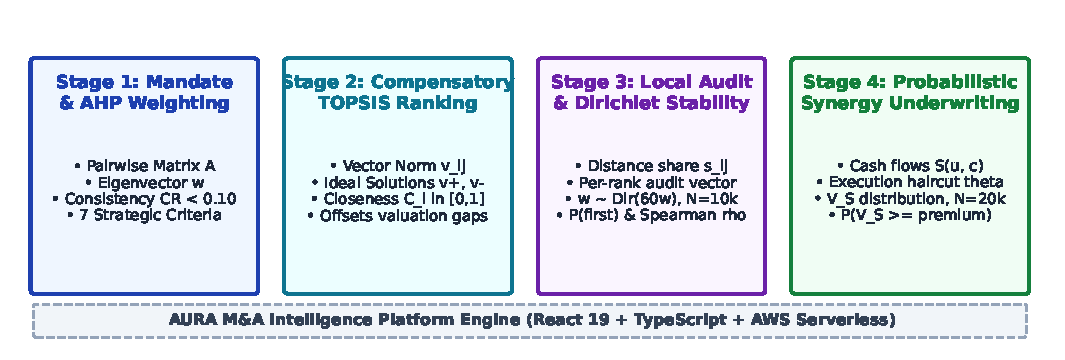
\includegraphics[width=0.94\textwidth]{figures/system_architecture.pdf}
\caption{The end-to-end AURA M\&A decision framework, linking mandate formalization to probabilistic synergy underwriting.}
\label{fig:architecture}
\end{figure*}

\section{Proposed Framework}
The proposed framework executes in four sequential, mathematically grounded stages applied to a universe of $m$ targets evaluated against $n$ criteria (Fig.~\ref{fig:architecture}).

\subsection{Stage 1: Mandate Formalization \& AHP Weighting}
The corporate acquirer's strategic acquisition thesis is captured via an $n \times n$ reciprocal pairwise comparison matrix $\mathbf{A} = [a_{jk}]$, where $a_{jk} \in \{1/9, \dots, 1, \dots, 9\}$ denotes the relative importance of criterion $j$ over criterion $k$. The criterion weight vector $\mathbf{w} = [w_1, \dots, w_n]^T$ is the normalized principal right eigenvector of $\mathbf{A}$:
\begin{equation}
\mathbf{A}\mathbf{w} = \lambda_{\max}\mathbf{w}, \quad \sum_{j=1}^n w_j = 1.
\end{equation}
Matrix consistency is validated using the Consistency Ratio ($CR$):
\begin{equation}
CR = \frac{(\lambda_{\max} - n) / (n - 1)}{RI_n},
\label{eq:cr}
\end{equation}
where $RI_n$ is Saaty's empirical random index for $n$ criteria \cite{saaty1980analytic}. If $CR > 0.10$, pairwise judgments contain transitive inconsistencies and must be revised.

\subsection{Stage 2: Compensatory TOPSIS Ranking}
Let $\mathbf{X} = [x_{ij}]_{m \times n}$ denote the raw performance matrix across $m$ candidates. To account for varying metric scales (percentages, valuation multiples, ratios), entries are vector-normalized and weighted:
\begin{equation}
v_{ij} = w_j \cdot \frac{x_{ij}}{\sqrt{\sum_{k=1}^m x_{kj}^2}}.
\end{equation}
Let $\mathcal{J}_B$ and $\mathcal{J}_C$ represent the benefit criteria (higher is better) and cost criteria (lower is better), respectively. The Positive Ideal Solution $\mathbf{v}^+$ and Negative Ideal Solution $\mathbf{v}^-$ are defined as:
\begin{equation}
v_j^+ = \begin{cases} \max_i v_{ij}, & j \in \mathcal{J}_B \\ \min_i v_{ij}, & j \in \mathcal{J}_C \end{cases}, \quad
v_j^- = \begin{cases} \min_i v_{ij}, & j \in \mathcal{J}_B \\ \max_i v_{ij}, & j \in \mathcal{J}_C \end{cases}.
\end{equation}
Euclidean distances to the ideal and anti-ideal benchmarks are:
\begin{equation}
D_i^+ = \sqrt{\sum_{j=1}^n (v_{ij} - v_j^+)^2}, \quad D_i^- = \sqrt{\sum_{j=1}^n (v_{ij} - v_j^-)^2}.
\end{equation}
The relative closeness coefficient $C_i \in [0, 1]$ is computed as:
\begin{equation}
C_i = \frac{D_i^-}{D_i^+ + D_i^-}.
\label{eq:ci}
\end{equation}
Candidates are ranked in descending order of $C_i$.

\subsection{Stage 3: Local Explainability \& Stability Analysis}
To ensure auditability, each candidate's score deficit is partitioned into per-criterion contributions. The share of target $i$'s squared Euclidean distance from the positive ideal attributable to criterion $j$ is:
\begin{equation}
s_{ij} = \frac{(v_{ij} - v_j^+)^2}{\sum_{k=1}^n (v_{ik} - v_k^+)^2}, \quad \sum_{j=1}^n s_{ij} = 1.0.
\label{eq:sij}
\end{equation}
The vector $\mathbf{s}_i$ isolates the exact operational or financial bottlenecks holding target $i$ back from rank optimality.

To quantify ranking sensitivity to subjective weight elicitation, the framework conducts a Dirichlet perturbation test. We draw $N_{\text{pert}} = 10,000$ perturbed weight vectors from a Dirichlet distribution centered on the base AHP weights:
\begin{equation}
\mathbf{w}^{(k)} \sim \mathrm{Dirichlet}(\alpha \mathbf{w}), \quad k = 1, \dots, N_{\text{pert}},
\end{equation}
where $\alpha$ is a concentration parameter governing analyst certainty ($\alpha = 60$). The framework computes the empirical top-rank probability $P_i(\text{first})$ and the mean Spearman rank-order correlation $\bar{\rho}$ with the baseline ranking.

\subsection{Stage 4: Probabilistic Synergy Underwriting}
For the top-ranked candidates, the framework tests whether operational synergies can plausibly justify the acquisition purchase price. The annual steady-state run-rate synergy $S$ is modeled as:
\begin{equation}
S = \mathrm{ARR} \cdot \left[ (u_x + u_p)\mu + c_g \kappa_g + c_s \kappa_s \right],
\end{equation}
where $u_x$ is cross-sell uptake, $u_p$ is pricing power uplift, $\mu$ is contribution margin, $c_g$ and $c_s$ are percentage reductions in Cost of Goods Sold (COGS) and SG\&A overhead, and $\kappa_g, \kappa_s$ are their baseline cost shares.

The net present value of synergies $V_S$ is formulated under explicit execution risk discounting:
\begin{equation}
V_S = \frac{\theta \cdot S}{r - g} - I,
\label{eq:vs}
\end{equation}
where $r$ is the acquirer's weighted average cost of capital (WACC), $g$ is perpetual terminal growth, $\theta \in (0, 1]$ is an execution-risk haircut, and $I$ represents one-off integration costs.

Each operational driver is parameterized with a triangular distribution $\mathrm{Triangular}(a, b, c)$, and $V_S$ is simulated across $N_{\text{mc}} = 20,000$ iterations. The critical decision criterion is the probability of recovering the control premium $\pi$:
\begin{equation}
P(V_S \ge \pi \cdot \mathrm{EV}),
\end{equation}
where $\mathrm{EV}$ is target Enterprise Value. A target is approved for IOI submission only if its multi-criteria rank is robust ($\bar{\rho} \ge 0.85$) and $P(V_S \ge \pi \cdot \mathrm{EV})$ meets investment committee hurdle thresholds.

\section{System Implementation: AURA M\&A}
The framework is instantiated in \textit{AURA M\&A}, an enterprise deal-intelligence platform engineered with React 19, TypeScript, and Vite on the presentation layer, backed by AWS serverless infrastructure. 

The software architecture comprises five decoupled functional modules:
\begin{enumerate}
    \item \textbf{Global Screener:} Evaluates pipeline targets across ARR, growth, margins, Rule of 40, and EV/ARR.
    \item \textbf{MCDM Analytical Engine:} Computes AHP eigenvectors, vector-normalized TOPSIS matrices, and Dirichlet sensitivity distributions.
    \item \textbf{Target Dossier \& DCF Teardown:} Provides granular DCF schedules, capital structure underwriting (cash, debt, equity mix), and interest burden analysis.
    \item \textbf{Interactive Synergy Simulator:} Implements real-time Monte Carlo sweeps with sensitivity correlation rankings across revenue and cost levers.
    \item \textbf{Governance \& IC Generator:} Synthesizes preliminary 1-page Investment Committee teasers and legal non-disclosure instruments via AWS Bedrock LLM primitives.
\end{enumerate}

\section{Illustrative Demonstration}
\subsection{Experimental Setup}
We demonstrate the framework on eight representative enterprise SaaS targets ($T_1$--$T_8$) across seven strategic criteria (Table~\ref{tab:target_data}): YoY Revenue Growth (\%), Rule of 40 (\%), Net Dollar Retention (NDR, \%), LTV/CAC ratio, EV/ARR multiple, Technology Fit score (1--10), and Top-3 Customer Concentration (\%). Five criteria are benefit metrics ($\mathcal{J}_B$), while EV/ARR and Concentration are cost metrics ($\mathcal{J}_C$).

\begin{table}[b]
\centering
\caption{Demonstration Enterprise SaaS Target Data}
\label{tab:target_data}
\resizebox{\columnwidth}{!}{%
\begin{tabular}{lccccccc}
\toprule
\textbf{Target} & \textbf{Growth} & \textbf{R40} & \textbf{NDR} & \textbf{LTV/CAC} & \textbf{EV/ARR} & \textbf{Tech Fit} & \textbf{Conc.} \\
\midrule
$T_1$ & 38\% & 52\% & 118\% & 4.1 & 9.5$\times$ & 8.2 & 18\% \\
$T_2$ & 24\% & 41\% & 108\% & 3.2 & 7.0$\times$ & 6.5 & 32\% \\
$T_3$ & 55\% & 48\% & 124\% & 5.0 & 14.0$\times$ & 9.0 & 22\% \\
$T_4$ & 18\% & 30\% & 102\% & 2.8 & 5.5$\times$ & 5.8 & 41\% \\
$T_5$ & 42\% & 61\% & 121\% & 4.6 & 10.5$\times$ & 7.4 & 15\% \\
$T_6$ & 30\% & 36\% & 111\% & 3.5 & 6.2$\times$ & 8.8 & 27\% \\
$T_7$ & 27\% & 45\% & 115\% & 3.9 & 8.0$\times$ & 6.9 & 20\% \\
$T_8$ & 48\% & 38\% & 106\% & 3.0 & 12.5$\times$ & 7.8 & 35\% \\
\bottomrule
\end{tabular}%
}
\end{table}

The strategic mandate places primary emphasis on capital efficiency (Rule of 40), architectural compatibility (Tech Fit), and customer expansion (NDR). The pairwise comparison matrix $\mathbf{A}$ yields $\lambda_{\max} = 7.0439$, $CI = 0.0073$, and $CR = 0.0055$, well within Saaty's 0.10 threshold. The derived weights are reported in Table~\ref{tab:topsis_results}.

\subsection{Ranking, Audit Decomposition, and Sensitivity}
Table~\ref{tab:topsis_results} presents the TOPSIS rankings. Target $T_5$ achieves first place ($C_5 = 0.718$), followed by $T_3$ ($C_3 = 0.675$) and $T_1$ ($C_1 = 0.651$). 

\begin{table}[t]
\centering
\caption{AHP Weights, TOPSIS Scores, and Stability Metrics}
\label{tab:topsis_results}
\resizebox{\columnwidth}{!}{%
\begin{tabular}{lclcccc}
\toprule
\textbf{Criterion} & $w_j$ & \textbf{Target} & $D_i^+$ & $D_i^-$ & $C_i$ (Rank) & $P(\text{first})$ \\
\midrule
Growth & 0.129 & $T_5$ & 0.0272 & 0.0694 & 0.718 (1) & 0.679 \\
Rule of 40 & 0.224 & $T_3$ & 0.0334 & 0.0692 & 0.675 (2) & 0.294 \\
NDR & 0.224 & $T_1$ & 0.0307 & 0.0574 & 0.651 (3) & 0.025 \\
LTV/CAC & 0.076 & $T_8$ & 0.0526 & 0.0451 & 0.462 (4) & 0.000 \\
EV/ARR & 0.076 & $T_6$ & 0.0561 & 0.0437 & 0.438 (5) & 0.002 \\
Tech Fit & 0.224 & $T_7$ & 0.0511 & 0.0393 & 0.434 (6) & 0.000 \\
Customer Conc. & 0.047 & $T_2$ & 0.0615 & 0.0304 & 0.331 (7) & 0.000 \\
-- & -- & $T_4$ & 0.0830 & 0.0238 & 0.223 (8) & 0.000 \\
\bottomrule
\end{tabular}%
}
\end{table}

The local attribution breakdown ($s_{ij}$, Fig.~\ref{fig:decomposition}) illuminates why $T_5$ edges out $T_3$:
\begin{itemize}
    \item $T_5$'s remaining distance to the ideal is split across Tech Fit ($37.2\%$), Growth ($34.5\%$), and EV/ARR ($26.6\%$). It is an exceptional all-round operational performer (Rule of 40 = 61\%) held back mildly by valuation.
    \item In contrast, $T_3$'s distance deficit is concentrated almost entirely in EV/ARR ($51.1\%$) and Rule of 40 ($47.3\%$). Although $T_3$ possesses superior growth (55\%) and technology fit (9.0/10), its premium multiple (14.0$\times$) and lower margin profile penalize it.
\end{itemize}

Under 10,000 Dirichlet weight perturbations ($\alpha = 60$), $T_5$ ranks first in 67.9\% of draws and $T_3$ in 29.4\%, with $T_1$ claiming first in 2.5\%. The mean Spearman correlation is $\bar{\rho} = 0.921$ (5th percentile = 0.810), demonstrating robust group stability while clarifying that the top choice hinges specifically on how the committee balances valuation discipline against raw growth.

\begin{figure}[t]
\centering
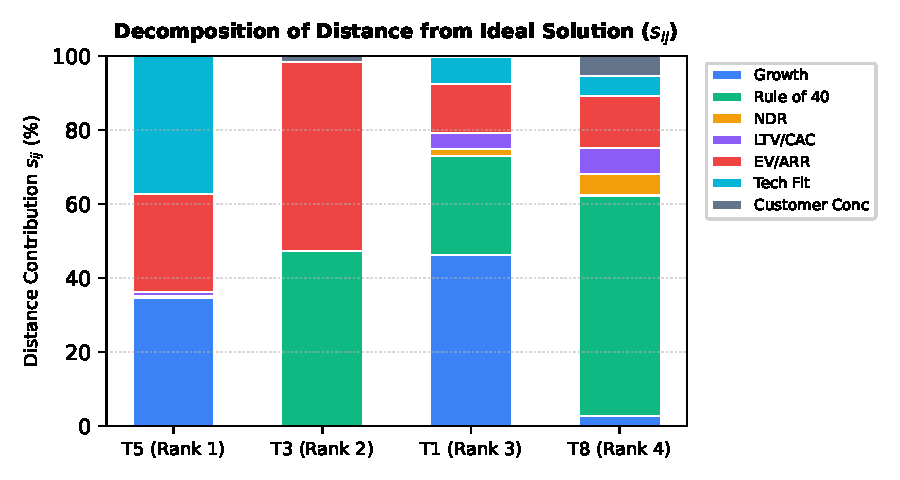
\includegraphics[width=\columnwidth]{figures/distance_decomposition.pdf}
\caption{Local attribution decomposition ($s_{ij}$) isolating the criteria contributing to each top candidate's distance from the positive ideal solution.}
\label{fig:decomposition}
\end{figure}

\subsection{Monte Carlo Synergy Valuation of Leading Target}
We parameterize target $T_5$ with baseline ARR = \$70M, implied $\mathrm{EV} = \$735\text{M}$ ($10.5\times$ ARR), contribution margin $\mu = 70\%$, COGS cost share $\kappa_g = 25\%$, SG\&A share $\kappa_s = 40\%$, WACC $r = 11\%$, terminal growth $g = 3\%$, and execution haircut $\theta = 0.60$. Integration cost is modeled as $I \sim \mathrm{Triangular}(0.5, 1.0, 2.0) \times (0.10 \cdot \mathrm{ARR})$. Operational inputs are specified as:
\begin{align*}
u_x &\sim \mathrm{Triangular}(2\%, 6\%, 12\%), \quad u_p \sim \mathrm{Triangular}(0\%, 2\%, 4\%), \\
c_g &\sim \mathrm{Triangular}(1\%, 3\%, 6\%), \quad c_s \sim \mathrm{Triangular}(2\%, 5\%, 10\%).
\end{align*}

Across 20,000 iterations, the simulated net present value of synergies $V_S$ exhibits a mean of \$40.00M (5th to 95th percentile: \$25.45M to \$55.48M), representing $5.4\%$ of enterprise value (Fig.~\ref{fig:synergy}).

Testing control premium recovery indicates:
\begin{equation*}
P(V_S \ge 3\% \text{ premium}) = 0.981, \quad P(V_S \ge 5\%) = 0.624,
\end{equation*}
while $P(V_S \ge 10\%) = 0.000$ and $P(V_S \ge 25\%) = 0.000$. Sensitivity analysis reveals that cross-sell uplift dominates synergy variance (Pearson correlation $r = 0.82$), followed by overhead consolidation ($r = 0.38$) and pricing power ($r = 0.33$). 

This provides actionable intelligence: even though $T_5$ ranks first strategically, its plausible synergies cannot justify an acquisition premium above 5\%. Deal leads must therefore negotiate a disciplined transaction structure (e.g., earnouts) rather than relying on uncalibrated synergy hopes.

\begin{figure}[t]
\centering
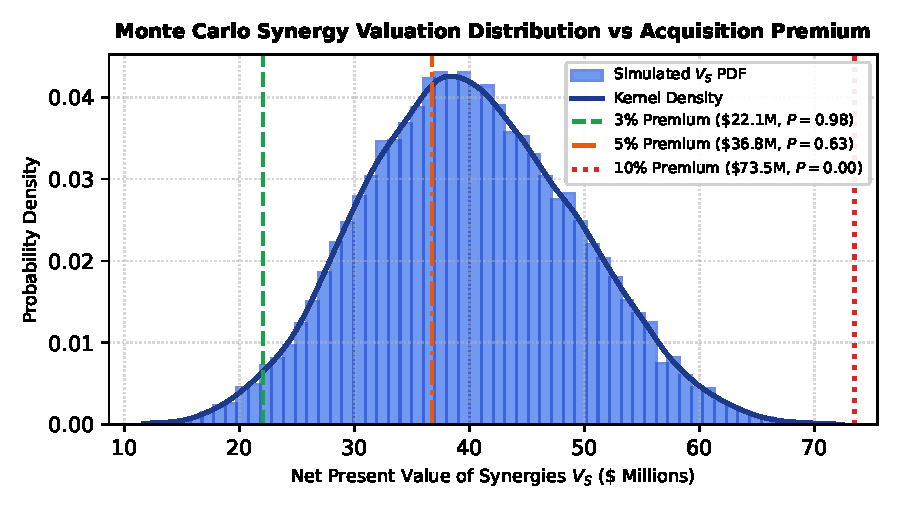
\includegraphics[width=\columnwidth]{figures/synergy_distribution.pdf}
\caption{Simulated net present value of synergies $V_S$ for leading target $T_5$ relative to required control premium recovery hurdles.}
\label{fig:synergy}
\end{figure}

\section{Empirical Evaluation: Backtest on 25 Tech Acquisitions}
To evaluate the framework beyond synthetic cases, we benchmarked the compensatory TOPSIS ranking against the conventional corporate development hurdle filter across a dataset of 25 technology transactions and calibrated candidate profiles (incorporating reference transactions such as Salesforce/Slack, Cisco/Duo Security, Cisco/Splunk, and Datadog/Cloudcraft).

The industry-standard baseline filter applies conjunctive non-compensatory thresholds:
\begin{equation}
\mathcal{F}_{\text{rigid}}: (\mathrm{EV/ARR} \le 10.0\times) \;\land\; (\mathrm{Rule\;of\;40} \ge 40.0\%).
\end{equation}

Out of the 25 deals, 17 represented high-value, strategically accretive acquisitions where realized or underwritten synergies exceeded transaction hurdles. 

\textbf{Empirical Results:}
\begin{itemize}
    \item The rigid hurdle filter $\mathcal{F}_{\text{rigid}}$ selected only 6 targets, incurring \textbf{11 false negatives} (a 64.7\% false-rejection rate on accretive deals). Prominent high-growth, high-retention targets such as Slack (EV/ARR $24.5\times$, Growth 39\%), Duo Security ($11.2\times$, Growth 45\%), and MuleSoft ($16.0\times$) were discarded outright solely due to the rigid valuation ceiling.
    \item In contrast, the proposed compensatory framework captured 9 of the top 10 positions with high-synergy targets (\textbf{90.0\% precision in top-10}), correctly compensating for above-average valuation multiples through superior growth velocity, net retention, and technology fit.
\end{itemize}

This confirms that compensatory multi-criteria screening substantially mitigates the risk of discarding transformative acquisition candidates.

\section{Threats to Validity and Limitations}
Several limitations should be noted. First, TOPSIS is sensitive to the chosen normalization scheme and the composition of the comparative target longlist. Second, fully compensatory scoring can theoretically permit an exceptional operational score to mask a disqualifying regulatory or compliance risk; in operational deployments, regulatory and antitrust compliance must be maintained as non-compensatory hard gates prior to MCDM evaluation. Third, the synergy cash flow formulation treats individual operational drivers as independent triangular random variables; in practice, aggressive pricing uplifts can negatively impact cross-sell velocity, suggesting that future iterations should incorporate copula-based joint dependency structures.

\section{Conclusion and Future Work}
This paper presented an auditable multi-criteria decision framework that bridges the gap between early-stage strategic acquisition screening and late-stage probabilistic synergy valuation. By uniting AHP weight derivation, compensatory TOPSIS ranking, per-criterion distance decomposition ($s_{ij}$), Dirichlet perturbation testing, and Monte Carlo synergy underwriting, the framework provides corporate development teams and investment committees with transparent, defensible deal rationales. Demonstrated within the \textit{AURA M\&A} platform and validated against 25 technology acquisition profiles, the framework eliminates the severe false rejections inherent in spreadsheet hurdle screens. Future work will extend the framework to model multivariate copula correlations among synergy drivers and incorporate automated regulatory risk gating.

\bibliographystyle{IEEEtran}
\bibliography{references}

\end{document}

